\section{Descripción TAMA}

Para construir la serie de tiempo de cada interlocutor, dividimos primero el diálogo en ventanas solapadas de igual tamaño \cite{KOU2008}. A la diferencia entre ventana y ventana llamaremos \emph{frame step}, y al tamaño de ventana \emph{frame length}.

\begin{figure}
\centering
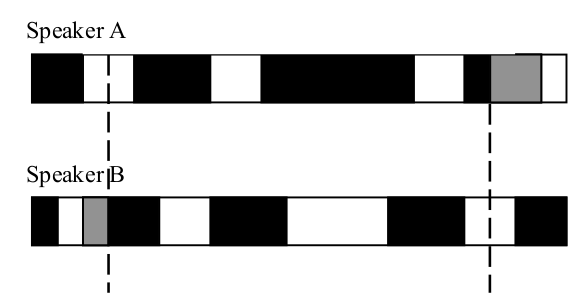
\includegraphics[width=10cm]{images/tama.png}

\end{figure}

Nuestro corpus está anotado de manera que tenemos separadas los intervalos donde los interlocutores hablan (llamaremos a cada uno de éstos locuciones o \emph{utterances}). Para cada una de los frames, calcularemos la media

\begin{align}
    \mu &= \sum\limits_{i=1}^N f_i dr_i \label{eq:tama_mean}\\
    dr_i &= \frac{d_i}{\sum\limits_{i=1}^N d_i} \\
\end{align}

donde $i$ itera sobre las locuciones dentro del \emph{frame}, $d_i$ es la duración de la locución y $f_i$ es el valor de la \emph{feature} que estamos midiendo.

Como se ve en \ref{eq:tama_mean}, el $\mu$ que calculamos es una media ponderada por la duración de las locuciones. Así, por ejemplo, al calcular una serie de tiempo sobre el \emph{pitch}, la contribución de interjecciones (usualmente de alto valor) estará disminuída por su breve duración.

La serie de tiempo constará entonces de la secuencia de medias calculadas con \ref{eq:tama_mean} para cada uno de los frames.


